\chapter{Localization}

\section*{Wheel Odometry}
\paragraph*{}
\quad Wheel odometry is solely calculated using the dynamic model of the omnidirectional wheeled robot. Hence, the position or the velocity of the wheel becomes a necessity. However, wheel odometry is only suitable under two conditions: the robot must not have wheel slip, and the encoder must be precise. 
\paragraph*{}
The problem that arose during the implementation phase was that the motor (Dynamixel AX-12W) was not able to return the complete position and velocity values. Due to the limited range of the embedded encoder in the motor, the resulting random value is between 330º and 350º (Figure \ref{fig:goal-position}). Moreover, the value returned by the encoder, according to the documentation, was the percentage of the maximum torque. \cite{robotisAX12W} 

\begin{figure}[H]
    \centering
    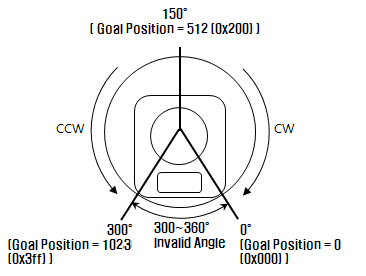
\includegraphics[width=0.35\linewidth]{assets/images/odometry/goal_position.png}
    \caption{Encoder diagram of AX-12W}
    \label{fig:goal-position}
\end{figure}

To work around this, we instead tried the current speed register. However, this approach requires the robot to operate at relatively low speeds to maintain accuracy. Yet, this method will not work during the collective transport phase, as the load to the motor will be different. Hence, LiDAR odometry was considered as the more viable solution for odometry.

\newpage
\section*{Odometry Validation}
\quad The performance evaluation of the LiDAR odometry is carried out using an overhead camera setup. To ensure that our odometry is accurate enough for use in SLAM, the camera tracks the robot’s movement and provides a ground-truth odometry reference. Then, the data from the camera are compared to the LiDAR's.

The testing was carried out in a controlled indoor environment using a Logitech C922 PRO HD Stream webcam mounted on a studio stand (Figure \ref{fig:camera-setting}). The tests were carried out on a flat surface free from slipperiness and reflections(Figure \ref{fig:arena-setting}). 
\begin{figure}[!htb]
    \centering
    \begin{minipage}{0.48\textwidth}
        \centering
        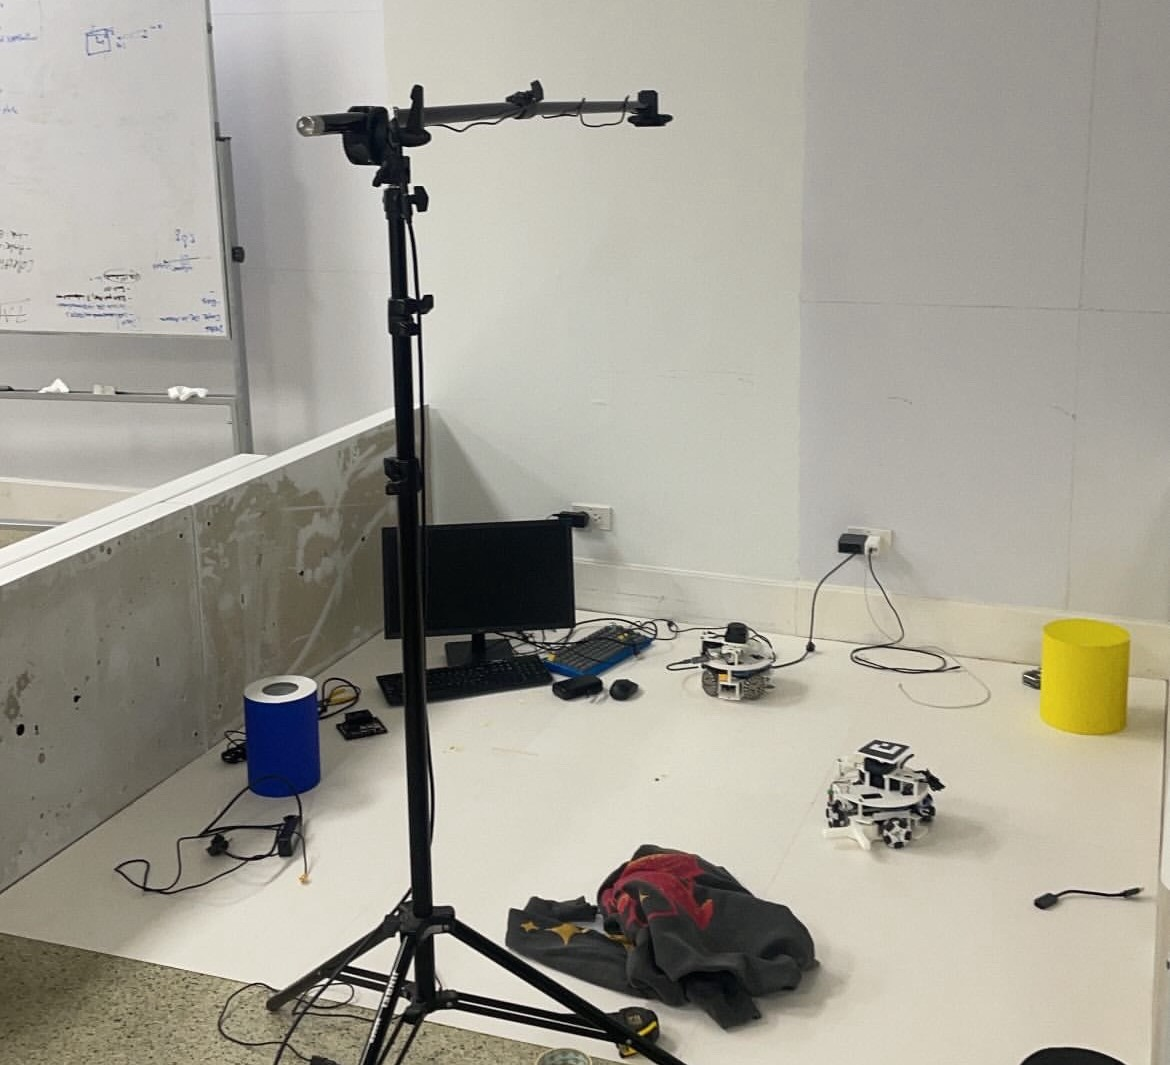
\includegraphics[height=3.5cm]{assets/images/odometry/cam_setting.jpg}
        \caption{Camera setup}
        \label{fig:camera-setting}
    \end{minipage}\hfill
    \begin{minipage}{0.48\textwidth}
        \centering
        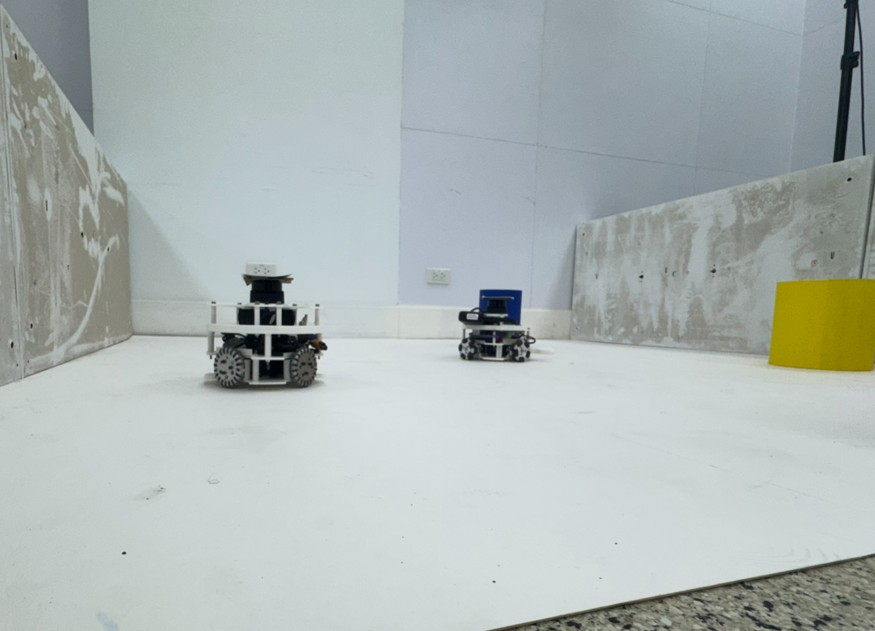
\includegraphics[height=3.5cm]{assets/images/odometry/arena_setting.jpg}
        \caption{Arena setup}
        \label{fig:arena-setting}
    \end{minipage}
\end{figure}

The Augmented Reality University of Cordoba (ArUco) markers are used to locate the robot's position within the testing arena. DICT\_4×4\_50 ArUco markers were selected for this testing because they're the least complex markers, making computation faster and more reliable for real-time detection. 

The ArUco markers were placed directly above the robot hardware, while the camera faced directly into the arena (Figure \ref{fig:aruco-swarm}). After that, our overhead camera system extracted the ArUcos from each camera frame and calculated the actual position from the map using the Perspective-n-Point (PnP) pose computation.

\begin{figure}[H]
    \centering
    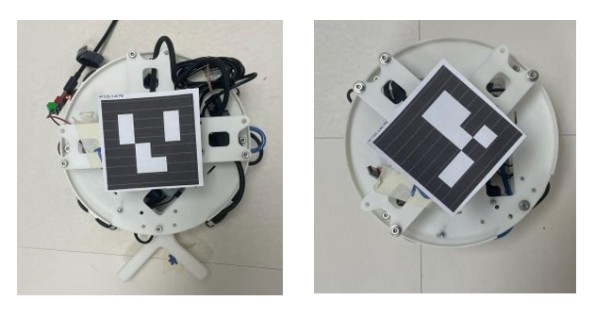
\includegraphics[width=0.35\linewidth]{assets/images/odometry/aruco.jpg}
    \caption{ArUco markers on the swarms}
    \label{fig:aruco-swarm}
\end{figure}

\subsection*{ArUco Marker Localization}

Given the four detected corner points of an ArUco marker in image coordinates:
\[
\text{Corners} = \{ \mathbf{p}_1, \mathbf{p}_2, \mathbf{p}_3, \mathbf{p}_4 \} = \{ \text{topLeft}, \text{topRight}, \text{bottomRight}, \text{bottomLeft} \}
\]

\paragraph*{1. Center of the Marker}
\[
c_x = \frac{x_{\text{topLeft}} + x_{\text{bottomRight}}}{2}, \quad
c_y = \frac{y_{\text{topLeft}} + y_{\text{bottomRight}}}{2}
\]

\paragraph*{2. Direction Vector of the Top Edge}
\[
\Delta x = x_{\text{topRight}} - x_{\text{topLeft}}, \quad
\Delta y = y_{\text{topRight}} - y_{\text{topLeft}}
\]

\paragraph*{3. Orientation Estimation}
Display orientation in degrees:
\[
\theta_{\text{display}} = \arctan2(\Delta y, -\Delta x)
\]

\paragraph*{4. Normalized Image Coordinates}
Assuming image width $W$ and height $H$:
\[
x_{\text{norm}} = \frac{c_x}{W}, \quad
y_{\text{norm}} = \frac{c_y}{H}
\]

\paragraph*{5. Real-World Position Mapping}
Given real-world map dimensions $S_x$ and $S_y$:
\[
x_{\text{map}} = (x_{\text{norm}} - 0.5) \cdot S_x, \quad
y_{\text{map}} = -(y_{\text{norm}} - 0.5) \cdot S_y
\]

The given formulation allows the transformation of detected 2D marker positions into real-world coordinates as figure shown:

\begin{figure}[H]
    \centering
    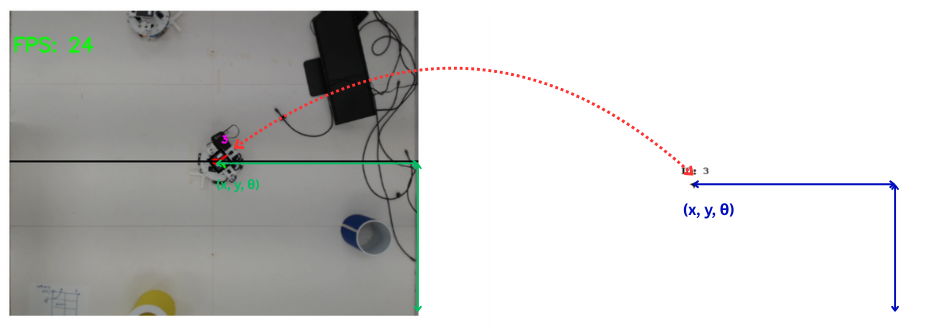
\includegraphics[width=1\linewidth]{assets/images/odometry/mapping.png}
    \caption{Visualization of real-time mapping of swarms using OpenCV and Turtle}
    \label{fig:coor-mapping}
\end{figure}

\newpage
After obtaining data from both the camera and LiDAR, we evaluated the trajectory error produced by the LiDAR odometry through the following tests:

\begin{enumerate}
    \item \textbf{Translational motion} (holonomic): The robot moved 50 cm in the positive \(x\)-direction via sideways motion (45° to the traveling direction).
    \item \textbf{Translational motion} (non-holonomic): The robot moved 50 cm in the positive \(x\)-direction via forward motion (0° to the traveling direction).
    \item \textbf{Rotational motion}: The robot performed a 360° turn clockwise and counterclockwise in place.
\end{enumerate}


\begin{figure}[H]
    \centering
    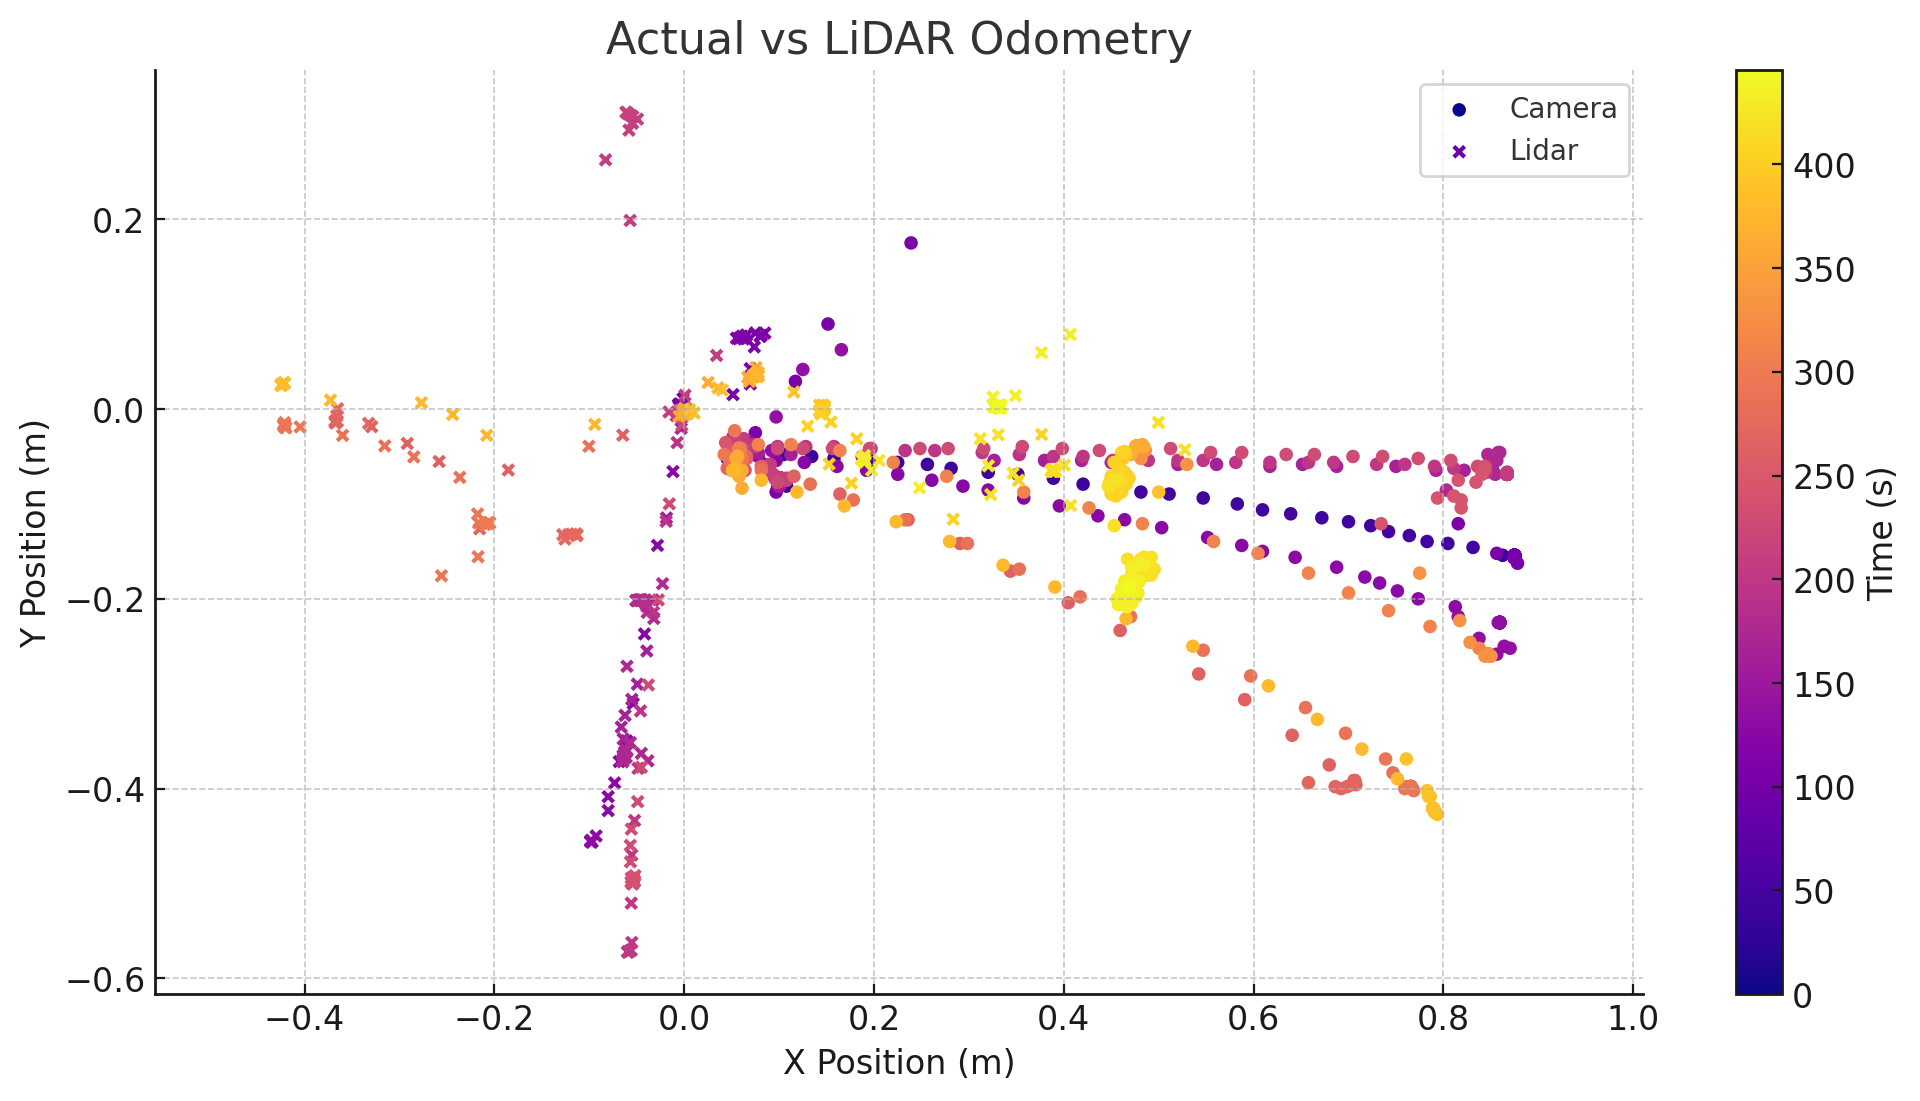
\includegraphics[width=0.7\linewidth]{assets/images/odometry/testing_visual.png}
    \caption{Visualization of robot motion based on LiDAR and camera odometry in a 2D plane.}
    \label{fig:visual-result}
\end{figure}

As shown in Figure\ref{fig:visual-result}, the robot’s ability to move in a straight line significantly deteriorated when switching from moving at a 45° angle to the direction of travel (using two wheels) to moving in the direction it is facing (using all four wheels). The goal of this analysis was to evaluate whether the LiDAR odometry could accurately capture trajectory errors and be reliably used for SLAM or feedback control.

However, one issue encountered was that LiDAR odometry assigned a different x-axis orientation for each test. To address this, we compensated for the discrepancy by remapping the x-axis to match the robot’s initial direction of motion during error calculation.

Figure\ref{fig:detail-result} presents the detailed numerical comparison of the robot's estimated position and orientation ($x$, $y$, and $\theta$) from both the LiDAR and camera odometry across all test scenarios.


\begin{figure}[H]
    \centering
    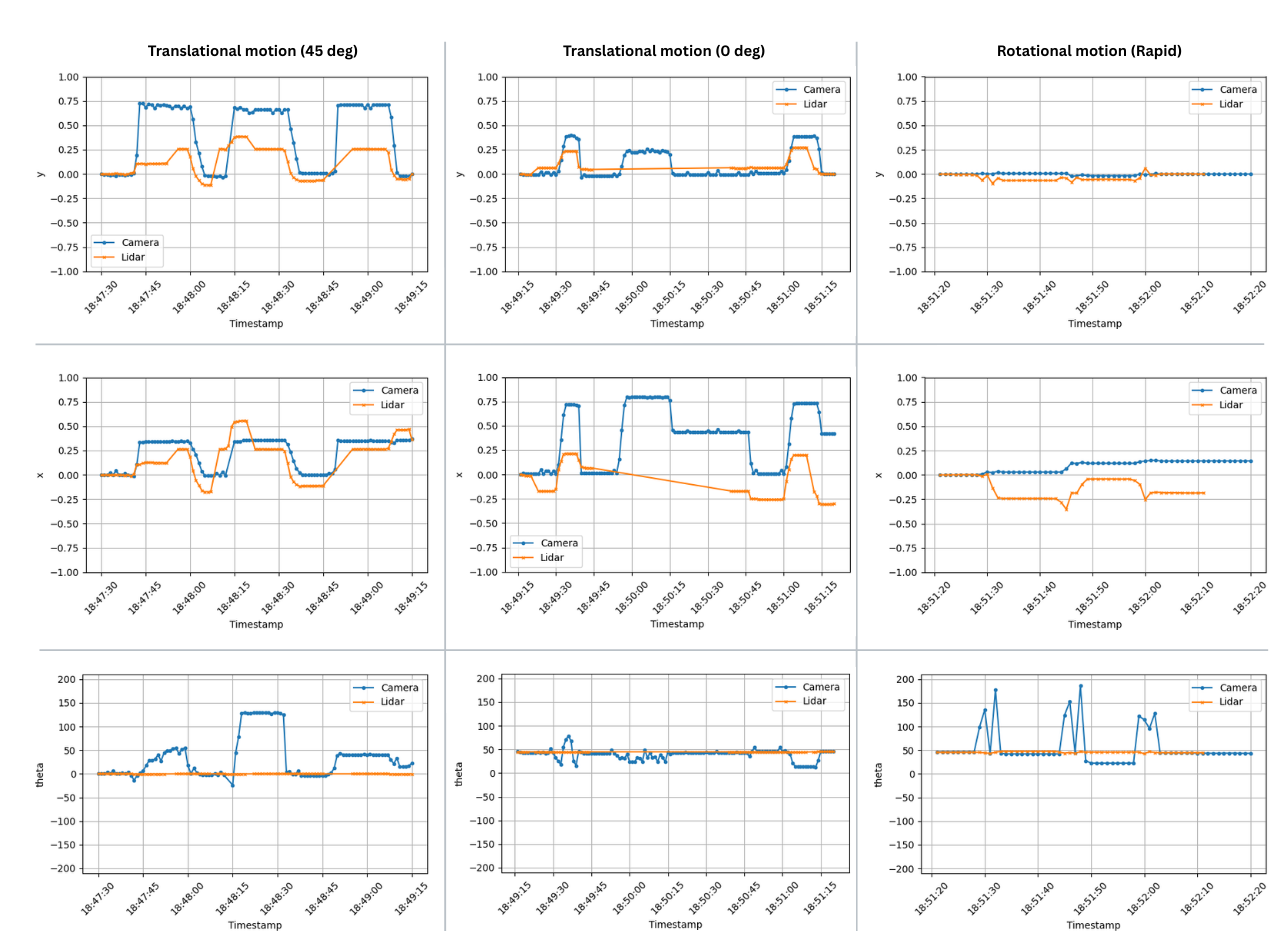
\includegraphics[width=1\linewidth]{assets/images/odometry/detail_visual.png}
    \caption{Detailed Visualization of LiDAR vs actual odometry}
    \label{fig:detail-result}
\end{figure}

\begin{table}[H]
\centering
\begin{tabular}{|c|c|c|c|}
\hline
\textbf{Metric} & \textbf{Translational (45°)} & \textbf{Translational (0°)} & \textbf{Rotational} \\
\hline
NRMSE (Y) & 0.483 & 0.597 & 1.282 \\
NRMSE (X) & 0.389 & 0.614 & 0.768 \\
NRMSE ($\theta$) & 0.360 & 0.629 & 0.407 \\
\hline
\end{tabular}
\caption{Normalised Root Mean Squared Error (NRMSE) Comparison Between Camera and LiDAR}
\label{tab:mse-results}
\end{table}

From our experiments, we observed that the current LiDAR odometry often deviates from the actual trajectory, especially in movements that involve rotation or sliding. These inconsistencies show that the LiDAR setup may not provide sufficient accuracy for precise localization tasks or feedback data. As a result, we propose using the overhead camera system with ArUco markers as a temporary but reliable substitute for ground-truth positioning. This approach offers improved consistency and will serve as our main reference until a more robust odometry solution is implemented.
